\section{Alimentação} % (fold)
\label{sub:alimentação}
	A equipe de engenharia de energia tem como meta desenvolver o sistema de alimentação para o funcionamento do robô aspirador. Existem diversas possibilidades de fornecer a energia necessária pra suprir a potência requerida pelo sistema, sendo que a mais usual seria a utilização de baterias, que podem ser sintetizadas como um conjunto de pilhas responsável por transformar energia química em energia elétrica, por meio de duas placas de composição diferente, chamadas eletrodos, sendo sempre um positivo e um negativo. 

	A fonte de alimentação ideal para o sistema segue alguns requisitos essenciais, como ter autonomia mínima de 30 minutos (tempo suficiente para aspirar um cômodo). Alguns parâmetros como tensão e corrente ainda não podem ser definidos nesta etapa do projeto. Buscando as alternativas disponíveis dentro desse universo nos deparamos com a opção das baterias NIMH, que apresenta uma gama com alguns modelos disponíveis e com valores variáves de tensão e corrente.
	
	A recarga dessas baterias varia de acordo com a potência fornecida por cada uma, no entanto alguns fabricantes produzem carregadores que retiram a tensão alternada de 220v, 60Hz para a tensão contínua da bateria escolhida. O manual do carregador informa o tempo máximo de recarga de 45 minutos para o modelo mais potente de bateria, número esse que pode ser de apenas 15 minutos em alguns casos. Dentre as opções disponíveis, estão dispostas três nas imagens abaixo (18v, 14.4v e 12.4v/ 3,3Ah e 2,6Ah).

	\begin{figure}[H]
		\centering
		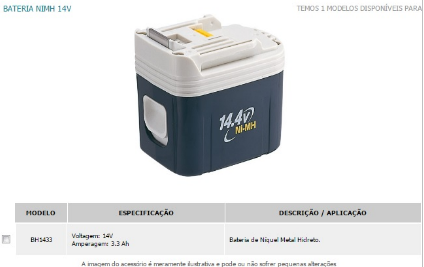
\includegraphics[scale=0.55]{figuras/bateria_1.png}
		\caption{Bateria de 14.4v.}
		\label{img:bateria_1}
	\end{figure}

	\begin{figure}[H]
		\centering
		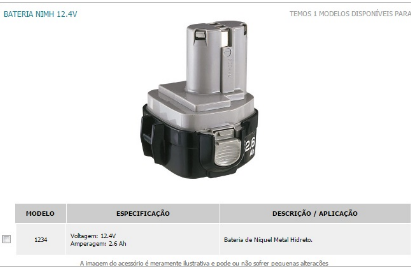
\includegraphics[scale=0.55]{figuras/bateria_2.png}
		\caption{Bateria de 12.4v.}
		\label{img:bateria_2}
	\end{figure}
	
	\begin{figure}[H]
		\centering
		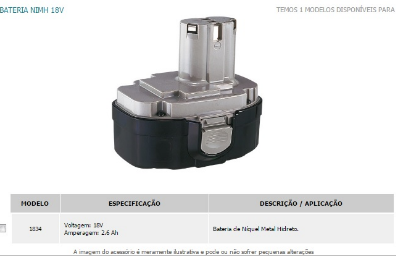
\includegraphics[scale=0.55]{figuras/bateria_3.png}
		\caption{Bateria de 18v.}
		\label{img:bateria_3}
	\end{figure}

	Uma outra alternativa para suprir a alimentação do aspirador seria o uso de supercapacitores. Tal opção oferece um valor consideravelmente maior de ciclos de carga (10 000 contra 400-6000), além um tempo de recarga muito reduzido se comparado com as baterias. Entre os fatores desfavoráveis pode-se citar a fragilidade, que acarreta em um maior cuidado no manuseio, o elevado custo de mercado além  da falta de informações técnicas obtidas até o momento.
% section alimentação (end)
